In leading order, we find
\begin{align}
c^{(0)}_{\tVV,F_2,\Pg} &= -\frac{\pi {\rho'}^3 }{4 \rho ^2 {\rho_q}^2}\left[2\beta\left(\rho ^2+{\rho_q}^2+\rho  {\rho_q} (6+{\rho_q})\right) \right.\nonumber\\
 &\hspace{50pt}\left.+\left(2 {\rho_q}^2+2 \rho  {\rho_q}^2+\rho ^2 (2-(-4+{\rho_q}) {\rho_q})\right) \ln(\chi)\right]\\
c^{(0)}_{\tVV,F_L,\Pg} &= -\frac{\pi{\rho'}^3}{\rho\rho_q}\left[2\beta + \rho\ln(\chi)\right]\\
c^{(0)}_{\tVV,2xg_1,\Pg} &= \frac{\pi{\rho'}^2}{2\rho\rho_q}\left[\beta(\rho+3\rho_q) + (\rho+\rho_q)\ln(\chi)\right]
\end{align}
\begin{align}
c^{(0)}_{\tAA,F_2,\Pg} &= \frac{\pi {\rho'}^3}{4\rho^2{\rho_q}^2}\left[ 2\beta\left(\rho ^2+{\rho_q}^2+\rho  {\rho_q} (6+{\rho_q})\right) \right.\nonumber\\
 &\hspace{50pt} \left. - \left(-6 \rho  {\rho_q}^2+2 (-1+{\rho_q}) {\rho_q}^2+\rho ^2 (-2+(-2+{\rho_q}) {\rho_q})\right) \ln(\chi) \right] \\
c^{(0)}_{\tAA,F_L,\Pg} &=-\frac{\pi{\rho'}^3}{2\rho^2\rho_q}\left[2\beta\rho(2+\rho_q) - \left(\rho ^2 (-1+{\rho_q})-4 \rho  {\rho_q}+{\rho_q}^2\right) \ln(\chi)\right]\\
c^{(0)}_{\tAA,2xg_1,\Pg} &= c^{(0)}_{\tVV,2xg_1,\Pg}
\end{align}
\begin{align}
c^{(0)}_{\tVA,xF_3,\Pg} &= c^{(0)}_{\tVA,g_4,\Pg} = c^{(0)}_{\tVA,g_L,\Pg} = 0
\end{align}

Near threshold we find
\begin{align}
c^{(0),\tThr}_{\tVV,F_2,\Pg} &= \frac{\pi\beta\rho_q}{2(\rho_q-1)}\\
c^{(0),\tThr}_{\tVV,F_L,\Pg} &= \frac{4\pi\beta^3\rho_q^2}{3(1-\rho_q)^3}\\
c^{(0),\tThr}_{\tVV,2xg_1,\Pg} &= c^{(0),\tThr}_{\tAA,2xg_1,\Pg} = c^{(0),\tThr}_{\tVV,F_2,\Pg}\\
c^{(0),\tThr}_{\tAA,F_2,\Pg} &= \frac{\pi\beta\rho_q^2}{1-\rho_q}\\
c^{(0),\tThr}_{\tAA,F_2,\Pg} &= \frac{\pi\beta(1-2\rho_q)\rho_q}{2(\rho_q-1)}
\end{align}

\begin{figure}[ht!]
\centering
\begin{subfigure}[t]{.3\textwidth}
	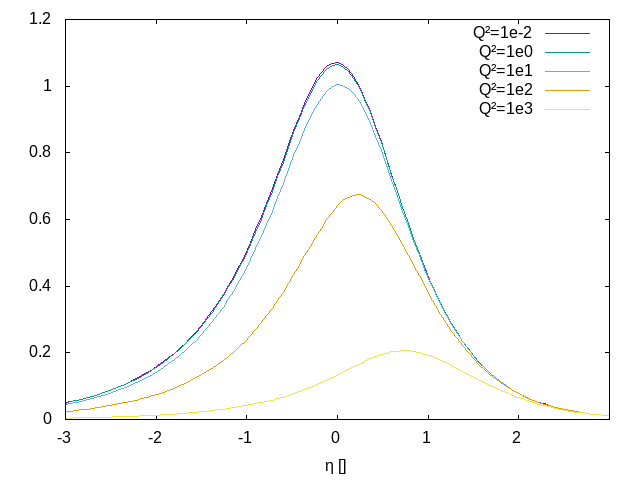
\includegraphics[width=\textwidth]{../../img2/partonic/cg0_VV_F2}
\end{subfigure}%
\begin{subfigure}[t]{.3\textwidth}
	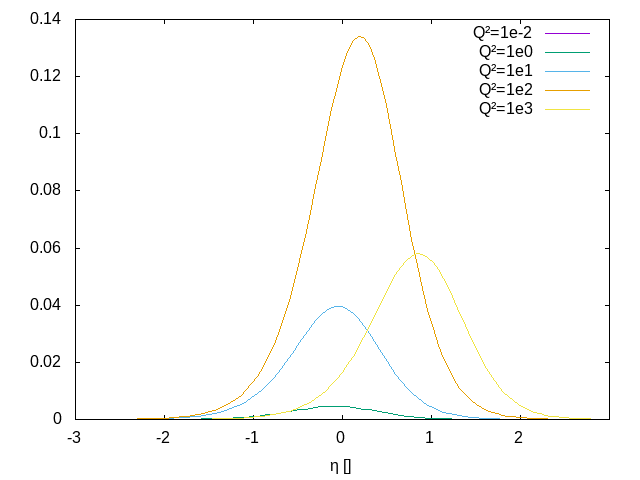
\includegraphics[width=\textwidth]{../../img2/partonic/cg0_VV_FL}
\end{subfigure}%
\begin{subfigure}[t]{.3\textwidth}
	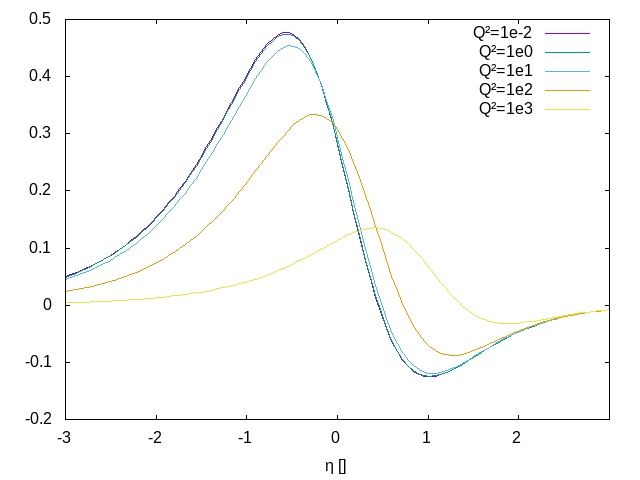
\includegraphics[width=\textwidth]{../../img2/partonic/cg0_VV_x2g1}
\end{subfigure}\\%
\begin{subfigure}[t]{.3\textwidth}
	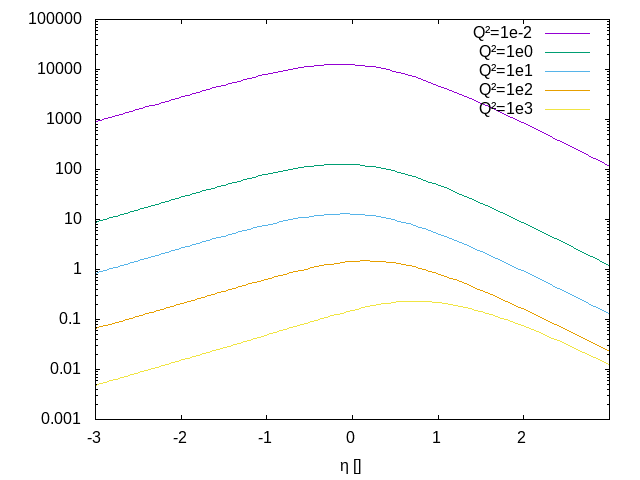
\includegraphics[width=\textwidth]{../../img2/partonic/cg0_AA_F2}
\end{subfigure}%
\begin{subfigure}[t]{.3\textwidth}
	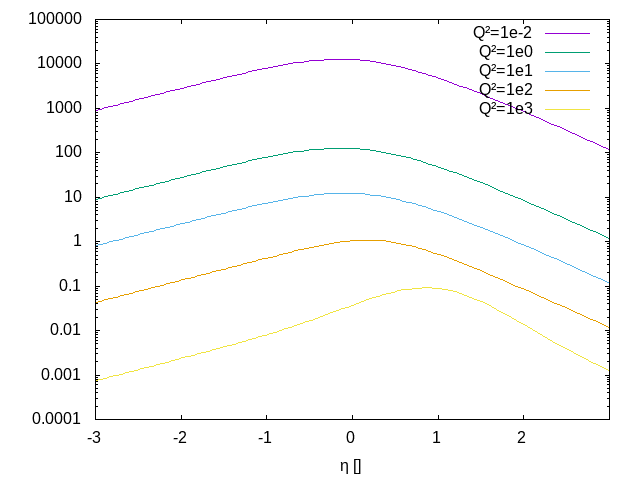
\includegraphics[width=\textwidth]{../../img2/partonic/cg0_AA_FL}
\end{subfigure}%
\begin{subfigure}[t]{.3\textwidth}
	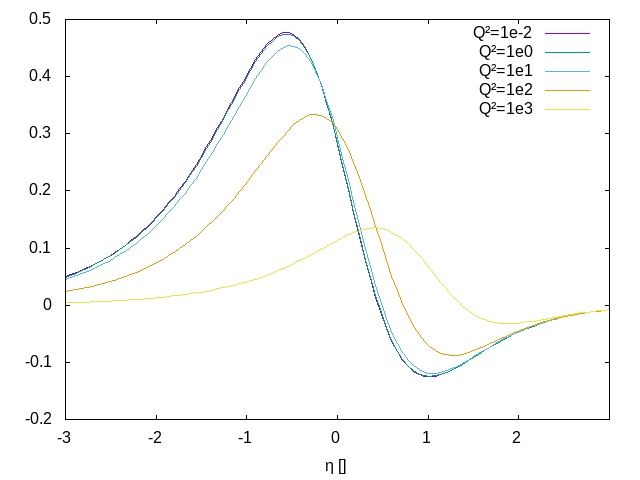
\includegraphics[width=\textwidth]{../../img2/partonic/cg0_AA_x2g1}
\end{subfigure}%
\caption{leading order scaling functions $c_{k,\Pg}^{(0)}(\eta,\xi)$ plotted as function of $\eta=s/(4m^2)-1$ for different values of $Q^2$ in units of $\si{\GeV^2}$ at $m=\SI{4.75}{\GeV}$ (i.e. different values of $\xi=Q^2/m^2$) }\label{fig:cg0}
\end{figure}
